\section{Wpływ reprezentacji stanu}
\label{sec:wyniki-reprezentacja-stanu}

W celu oceny wpływu sposobu reprezentacji stanu porównałem warianty
RAW i FEATURES przy zachowaniu tego samego algorytmu, funkcji nagrody
oraz seedu treningowego. Dla każdej pary wyznaczyłem różnicę

\begin{equation}
    \Delta EV_{\mathrm{state}}
    =
    EV_{\mathrm{FEATURES}}
    -
    EV_{\mathrm{RAW}}.
\end{equation}

Zgodnie ze wzorem dodatnia wartość różnicy oznacza zatem przewagę reprezentacji
FEATURES. Porównanie wykonałem osobno dla obu algorytmów i obu funkcji
nagrody. Jednostką porównania jest w tym przypadku seed treningowy,
dlatego każda wartość średnia oraz odpowiadający jej przedział ufności
wynikają z pięciu sparowanych różnic.

Wyniki wszystkich czterech porównań przedstawiam
w tabeli~\ref{tab:state-representation-effect}.

\begin{table}[htbp]
    \centering
    \caption{Wpływ reprezentacji stanu na EV}
    \label{tab:state-representation-effect}
    \begin{tabular}{llrr}
        \toprule
        Algorytm & Nagroda & $\Delta EV_{\mathrm{state}}$ & 95\% CI \\
        \midrule
        DQN & zysk netto
            & 0{,}2374 & [0{,}2066,\ 0{,}2682] \\
        DQN & skalowana
            & 0{,}1517 & [0{,}0863,\ 0{,}2170] \\
        \midrule
        REINFORCE & zysk netto
            & -0{,}0037 & [-0{,}0144,\ 0{,}0069] \\
        REINFORCE & skalowana
            & 0{,}0593 & [-0{,}0225,\ 0{,}1411] \\
        \bottomrule
    \end{tabular}
\end{table}

W przypadku DQN zastosowanie reprezentacji FEATURES doprowadziło do
wyraźnej poprawy końcowego EV dla obu funkcji nagrody, w obu przypadkach
cały przedział ufności leży powyżej zera. Wynika z tego, że w badanej
konfiguracji DQN rozszerzenie wektora stanu o cechy opisujące sytuację
pokerową poprawiało jakość uzyskiwanej strategii.

Dla REINFORCE wpływ reprezentacji stanu był znacznie mniej jednoznaczny.
Przy funkcji nagrody opartej na zysku netto przedział ufności obejmował
zero, dlatego na podstawie tych pięciu par nie mogę wskazać wyraźnej
przewagi żadnej z reprezentacji. Przy skalowanej funkcji nagrody
punktowe oszacowanie wskazuje na wyższe EV reprezentacji FEATURES,
jednak przedział ufności jest znacznie szerszy i również obejmuje zero,
więc duże zróżnicowanie wyników między seedami nie pozwala mi uznać tego
efektu za równie stabilny jak w przypadku DQN.

Te same porównania przedstawiam także na
rysunku~\ref{fig:state-representation-effect}, gdzie na osi poziomej
znajduje się różnica $EV_{\mathrm{FEATURES}} - EV_{\mathrm{RAW}}$,
a na osi pionowej cztery kombinacje algorytmu i funkcji nagrody.
Punkty przedstawiają średnią różnicę dla pięciu sparowanych seedów
treningowych, a wąsy odpowiadają 95-procentowym przedziałom ufności,
wartości dodatnie oznaczają przewagę reprezentacji FEATURES. Widać, 
że przedziały ufności obu wariantów DQN leżą całkowicie po
dodatniej stronie zera, natomiast oba przedziały REINFORCE obejmują
zero.

\begin{figure}[htbp]
    \centering
    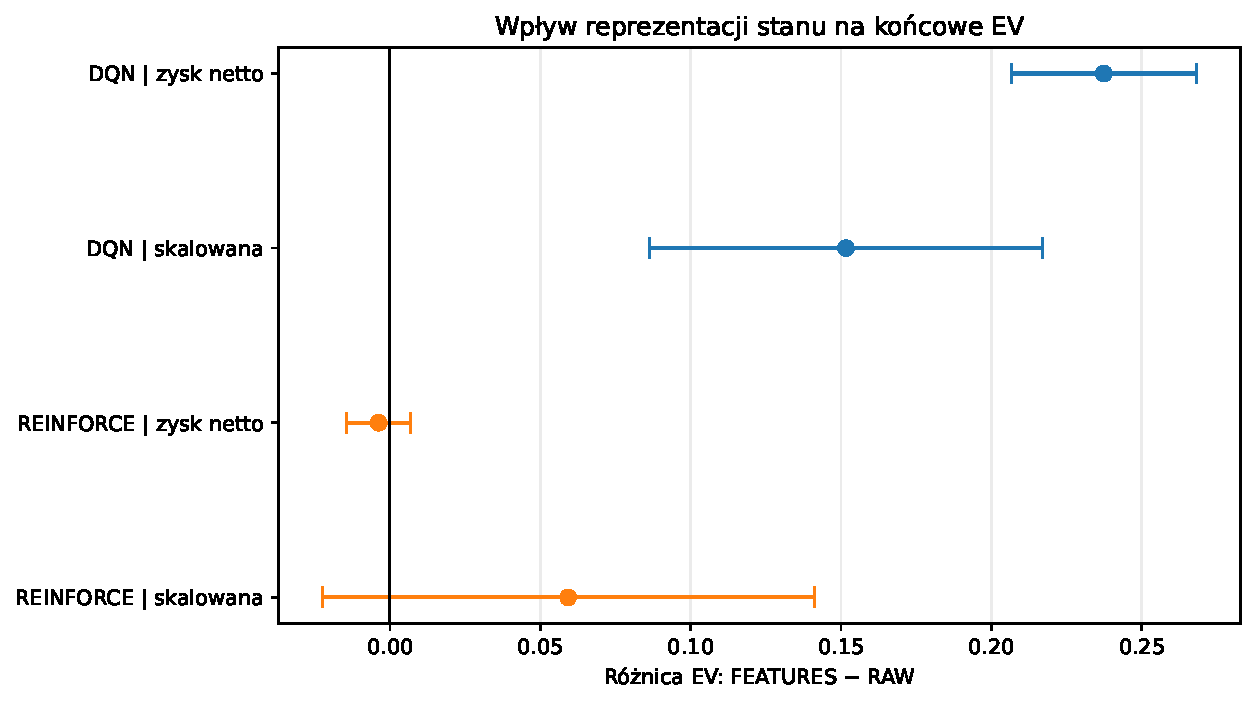
\includegraphics[
        width=0.9\textwidth
    ]{../experiments/results/final_analysis/02_state_representation_effect.pdf}
    \caption{Wpływ reprezentacji stanu na końcowe EV.}
    \label{fig:state-representation-effect}
\end{figure}

Rezultaty wskazują na odmienny wpływ reprezentacji
stanu na oba badane algorytmy. DQN korzystał z informacji zawartych
w rozszerzonej reprezentacji FEATURES, natomiast dla REINFORCE
nie zaobserwowałem równie stabilnego efektu zmiany reprezentacji.
